\documentclass[../MaxHughesThesis.tex]{subfiles}

\begin{document}

The standard model of particle physics can be tested in several ways.
For precision measurements, a careful measurement of a parameter thought to be zero is done.
If a non-zero result is found, new physics is discovered.
A window for low energy precision measurements is through beta decay.
Low-energy measurements are not the only method to look for new physics.

The most direct way to look for new physics is to create and detect new particles.
This is done with high energy experiments. 
The direct detection of new particles is very general and a powerful technique, as any avenue with a new particle can be probed.
However, high enough energy is needed to create the particle.
Precision measurements at high energies with colliders are often done as well. 
 
Low energy precision measurements, on the other hand, are much more specialized.
Precision measurements are sensitive to only certain channels of new physics.
Care must be taken that the channel of physics is not covered by collider experiments already.
For nuclear physics searches, this can be done by looking at beta decay, which provides a sensitive probe to several avenues of new physics.

\section{Beta Decay}
Beta decay is one of the processes by which unstable nuclei transform. 
The general process is %shown in equation \ref{eq:betadecay}

\begin{equation}
	\label{eq:betadecay}
	^{A}_{Z}P \rightarrow ^{A}_{Z\pm 1}D + e^{\mp} + \nu_{e}
\end{equation}
with $^{A}_{Z}P$ being the parent nucleus, $^{A}_{Z \pm 1}D$ being the daughter nucleus, $e^{\mp}$ is the outgoing electron or positron, and $\nu$ is an outgoing neutrino.
This is an anti-electron neutrino in the case of beta$^{-}$ decay, and an electron neutrino in the case of beta$^{+}$ decay. 
A related process is electron capture, where a proton in the nucleus captures an inner electron and turns into a neutron.

The simplest type of nuclear beta decay is allowed beta decay.
There are two types of allowed beta decay, which differ in angular momentum $J$ and isospin $T$ selection rules.
These are called Fermi and Gamow-Teller transitions. 
For a Fermi transition, the change of the angular momentum $J$ and the change of the isospin $T$ are both zero.
For a Gamow-Teller transition, the change in the angular moment $J$ is $0$ or $\pm1$ and the change of the isospin $T$ is $0$ or $\pm 1$.
However, a Gamow-Teller transition cannot cause a transition between two states of $J = 0$. 
These are called super-allowed beta decays.
There are also mixed allowed transitions, where both matrix elements of Fermi decay and Gamow Teller decay contribute.
In order to see what physics beyond the standard model beta decay measurements are sensitive to, a closer look at beta decay is needed.

\subsection{Microscopic View of Beta Decay}
At a microscopic level, the process of beta decay involves one of the quarks inside the nucleon emitting a $W$ boson. 
This quark changes flavor, and the nucleon changes as well. 
The microscopic view of beta decay (for the beta$^{-}$ case) is shown in figure \ref{fig:betadecaymicro}.

\begin{figure}[!htb]
	\centerline{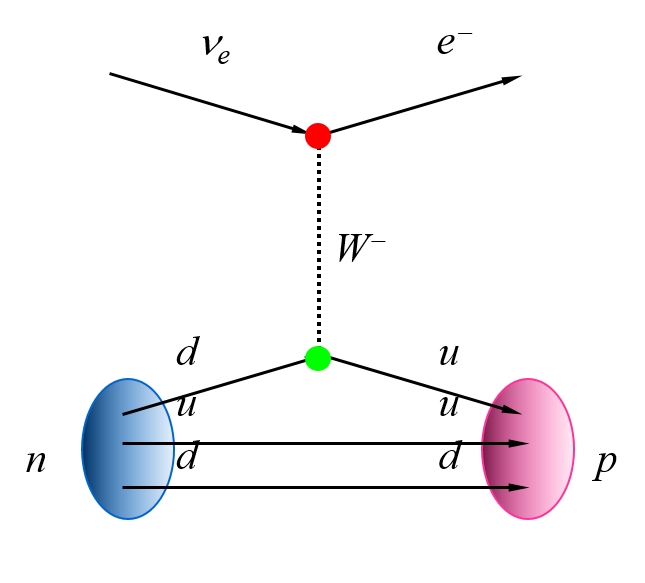
\includegraphics[width=0.5\textwidth]{fig_betadecayzoomedin.png}}
	\caption{What beta$^{-}$ decay looks like microscopically.}
	\label{fig:betadecaymicro}
\end{figure}
A down quark in a neutron goes to an up quark.
This process emits a $W^{-}$ boson that decays into an electron and an anti-electron neutrino.
Measurements of beta decay are complementary to high energy measurements of weak interactions.
For this work, a nucleon level treatment of beta decay will suffice.  

\subsection{Beta Energy Spectrum}
In order to determine the observables in beta decay, the energy spectrum must be written down. 
The spectrum is %shown as in equation \ref{eq:fgr}.
\begin{equation}
	\frac{dE}{dN} = PS(E) \times C(E) \times W(E)  
	\label{eq:betaenspectrum}
\end{equation}
The phase space, $PS(E)$, and the corrections, $C(E)$, will be discusses further in the thesis. 
The contributions from the weak interaction, $W(E)$ are to first order \cite{Jack57} %shown in equation \ref{eq:matrixelement} \cite{Gon19}
\begin{equation}
	 W(E) = \xi [1 + a \frac{\vec{p_{e}} \cdot \vec{p_{\nu}}} {E_{e} E_{\nu}}  +  b \frac{m_{e}}{E_{e}} + \frac{\vec{<J>}}{J} \cdot (A \frac{ \vec{p_{e}} }{E_{e}} + B \frac{\vec{p_{\nu}}}{E_{\nu}} + D \frac{\vec{p_{e}} \times \vec{p_{\nu}}}{E_{e} E_{\nu}})]
	\label{eq:matrixelement}
\end{equation}
$\xi$ is written out to linear order is %in equation \ref{eq:xiwrittenout}. 
 
\begin{equation}
	\xi = \frac{1}{2} |M_{F}|^{2} |C_{V} + C'_{V}|^{2} (1 + |\rho|^{2})
	\label{eq:xiwrittenout}
\end{equation}
where $M_{F}$ is the Fermi matrix element, $C_{V}$ and $C_{V}'$ are vector coupling constants, and $|\rho|$ is the ratio of the Gamow-Teller matrix element to the Fermi matrix element times $g_{A}/g_{V}$.
In equation \ref{eq:matrixelement}, $<\vec{J}>$ is the average total angular momentum. 
The constants $a$, $b$, $A$, $B$, and $D$ can be written in terms of the coupling constants.
The $\vec{p_{i}}$ are the momenta of the particles, and the $E_{i}$ the energies of those particles.
$a$ depends on the ratio of the Fermi and Gamow-Teller matrix elements $\rho$.
The functional form of equation \ref{eq:matrixelement} informs the experimental design.

\section{Types of Precision Measurements in Beta Decay}
To measure the terms in equation \ref{eq:matrixelement}, different types of experiments are needed.
To extract $a$, both the direction of the neutrino momentum $\vec{p_{e}}$ and $\vec{p_{\nu}}$ are needed.  
The direction of electron momentum is measured directly. 
The direction of the neutrino momentum is calculated from the electron momentum and the momentum of the recoiling daughter nucleus. 
To measure $A$, $B$, or $D$, a polarized nucleus is needed.
This points $<\vec{J}>/J$ in one direction, and then the corresponding momentum is measured.
To measure $A$, for example, the direction of the outgoing electrons is measured.
This direction corresponds to $AP\cos{\theta}$, where $P$ is the polarization fraction and $\theta$ the direction of the electron momentum.
Many more correlations exist at higher orders.

For an unpolarized nucleus where only the energy of the electron is measured, the momenta are averaged over and all terms in equation \ref{eq:matrixelement} disappear except for $b$.
There are two general kinds of unpolarized beta decay measurements.
The first is where the differential energy spectrum is measured.
There is a measurement of $b$ over the entire range of values, and the entire $1/W$ dependence is probed.
To do this measurement, the beta decay in question must be available enough in order to get enough statistics for a good spectrum.
Other requirements for a spectrum shape measurement are described in the next chapter.

To extract the Fierz term, b, electromagnetic and hardonic corrections are needed.
For the shape measurements, the energy dependence of the corrections are important.
Getting a better measurement of this term is one of the goals of this work.

\subsection{Fierz Term}
The Fierz term, $b$, in equation \ref{eq:matrixelement}, can be rewritten in terms of effective couplings.
This is %shown in equation \ref{eq:bwrittenout}

\begin{equation}
	b =  \pm 2 \sqrt{1 - \alpha^{2}{Z^{2}}}\frac{1}{1 + |\rho|^{2}}Re(\frac{C_{S} + C_{S}'}{C_{V} + C_{V}'} + |\rho|^{2}\frac{C_{T} + C_{T}'}{C_{A} + C_{A}'})
	\label{eq:bwrittenout}
\end{equation}
where $\alpha$ is the fine structure constant \cite{Jack57}.
The positive sign corresponds to electron decay and the negative sign to positron decay.  
The subscripts of $C$ indicate which object the coupling corresponds to. 
Here, $A$ stands for axial vector, $V$ stands for polar vector, $S$ stands for scalar, and $T$ stands for tensor. 
The $C$ coefficients correspond to parity conserving interactions, and the $C'$ coefficients correspond to parity non-conserving coefficients \cite{Lee56}
This means, that in a pure Fermi decay, the Fierz term is sensitive to any non-standard scalar term, while in a pure Gamow-Teller decay, the Fierz term is sensitive to any non-standard Tensor term. 

\subsubsection{Previous Fierz Term Measurements}
The Fermi decays have been measured using super-allowed beta decays.
The $ft$ value was measured, which is the integral of the decay spectrum $f$ times the partial half-life $t$.
The partial half-life is the half-life times the branching ratio.
This gives a value of $b$ modulated by the average value of $1/W$.
From the supperallowed beta decays, the result for the Fierz term is $-0.0028 \pm 0.0026$ \cite{Har17}.
It was obtained with $ft$ measurements of 14 different nuclei.
The uncertainty is the statistical uncertainty of the fit after the $ft$ values were corrected.
However, this Fierz term is sensitive to scalar couplings.
It took 14 different measurements to come up with this number.
The other part of the Fierz term is the tensor coupling. 

A spectrum shape measurement was done with ultra-cold neutrons \cite{Hic17}.
The beta energy spectrum was measured using a magnetic spectrometer.
The neutrons were confined in the center with a magnetic field, and allowed to decay.
A superratio was used to extract the Fierz term.
With the systematic effects, the final results of the Fierz term was $0.067 \pm 0.005_{stat}$ $ ^{+0.090}_{-0.061} sys$.
A sample beta spectrum is shown in figure \ref{fig:ucnabeta}.

\begin{figure}[!htb]
        \centerline{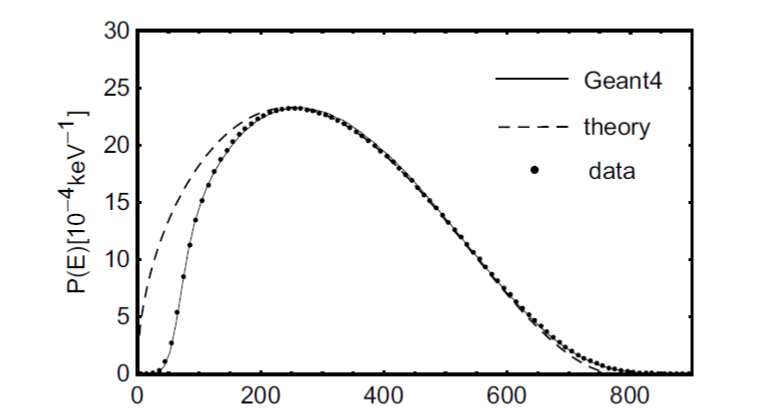
\includegraphics[width=0.78\textwidth]{NeutronBetaSpectrumUCNA.png}}
        \caption{The energy spectrum of the ultra-cold neutron measurement \cite{Hic17}. }
        \label{fig:ucnabeta}
\end{figure}

There are large distortions at low energy due to back-scattering effects.
Since the decay of a neutron is a mixed decay, this Fierz term is sensitive to both the tensor couplings and the scalar couplings.
In order to get a good measurement of  tensor couplings, an allowed Gamow-Teller decay must be used. 
The nucleus for this measurement was $^{20}$F.

\subsection{High Energy Probes of the Tensor Couplings} 

There are probes sensitive to the same physics as in Fierz term done with high energy techniques \cite{Gon19}.
The precision of these measurements is important to keep in mind, as this is the precision goal of the beta decay measurement.
Several high-energy channels are used, and the coupling constants are directly measured.
To compare the results of the channels to a precision beta decay measurement, the Fierz terms needs to be rewritten.
In the case of a Gamow-Teller transition, the Fierz term in equation \ref{eq:bwrittenout} can be re-written as %equation \ref{eq:bgt}

\begin{equation}
	b_{GT} = \pm 2 \sqrt{1 - \alpha^{2} Z^{2}} Re(\frac{C_{T} + C_{T}'}{C_{A} + C_{A}'})
	\label{eq:bgt}
\end{equation}
In terms of the quark level coupling constants, this can be rewritten as \cite{Gon19} %shown in equation \ref{eq:bgtquarklevel} \cite{Gon19}

\begin{equation}
	b_{GT} = \pm 2 \sqrt{1 - \alpha^{2} Z^{2}} Re(\frac{8 g_{T} \epsilon_{T}}{2 g_{A}})
	\label{eq:bgtquarklevel}
\end{equation}
with $g_{T}$ being the tensor charge, $\epsilon_{T}$ the tensor coupling and $g_{A}$ the axial vector charge.
This is assuming the only physics beyond the standard model is in $\epsilon_{T}$.
The value of $g_{T} = 0.987(55)$ and $g_{A} = 1.278 (33)$ \cite{Gon19}.
This means, for $^{20}$F, the value to $b_{GT}$ in terms of $\epsilon_{T}$ is given by %equation \ref{eq:bgtpropor}

\begin{equation}
	b_{GT} = \pm 6.2 \times Re(\epsilon_{T})
	\label{eq:bgtpropor}
\end{equation}
This can be used to describe the ultimate sensitivity needed.

For the high energy probes, the Large Hadron Collider collides two protons and looks at the output. 
The experimental signature for the LHC is missing transverse energy.
The energy of the output particles is compared to that of the standard model background, and the difference recorded.
To probe the same physics as beta decay, one or more of the outgoing particles are electrons or positrons.
For events with one electron and other particles, the constraint is $|\epsilon_{T}| < 1.3 \times 10^{-3}$.
Looking at neutral currents, where the output particles include an electron and a positron, gives stronger constraints.
There, the constraint is $|\epsilon_{T}| < 0.6 \times 10^{-3}$.
To be competitive with the stronger constraint from high energy experiments, the Fierz term $b_{GT}$ should be measured to better than $3.7 \times 10^{-3}$, assuming that $\epsilon_{T}$ is real. 

In order to achieve such a sensitivity, the technique used was a shape measurement.

\end{document}
